% !TeX spellcheck = en_GB
\ifcsname SlidesDistr\endcsname%
	\documentclass[handout,aspectratio=169]{beamer}
\else%
	\documentclass[aspectratio=169]{beamer}
\fi%
\usepackage{fontspec}
\usepackage[T1]{fontenc}
\usepackage{amsmath}
\usepackage{amsfonts}
\usepackage{amssymb}
\usepackage{graphicx}
\usepackage{csquotes}
\usepackage{booktabs}
\usepackage{multicol}
\usepackage{enumerate}
\usepackage{microtype}
\usepackage[labelfont=bf,font={small}]{caption}
\usepackage{hyperref}
\usepackage{booktabs}
\usepackage{subcaption}
\usepackage{fancyhdr}
\usepackage{pdfpages}
\usepackage{siunitx}
\usepackage{tikz}
\usepackage{mdframed}

\defaultfontfeatures{Mapping=tex-text}
\newfontfamily\symbolfont{Symbola}
\newfontfamily\quotefont{Gentium}

\usepackage[sorting=none]{biblatex}
\addbibresource{../bibliography.bib}

\author{Andreas Stöckel}


\renewcommand{\vec}[1]{{\mathbf{#1}}}
\newcommand{\mat}[1]{{\mathbf{#1}}}
\newcommand{\T}{\ensuremath{\mathsf{T}}}
\renewcommand{\epsilon}{\varepsilon}
\renewcommand{\phi}{\varphi}

% Tango color palette
\definecolor{butter1}{HTML}{FCE94F}
\definecolor{butter2}{HTML}{EDD400}
\definecolor{butter3}{HTML}{C4A000}
\definecolor{orange1}{HTML}{FCAF3E}
\definecolor{orange2}{HTML}{F57900}
\definecolor{orange3}{HTML}{CE5C00}
\definecolor{chocolate1}{HTML}{E9B96E}
\definecolor{chocolate2}{HTML}{C17D11}
\definecolor{chocolate3}{HTML}{8F5902}
\definecolor{chameleon1}{HTML}{8AE234}
\definecolor{chameleon2}{HTML}{73D216}
\definecolor{chameleon3}{HTML}{4E9A06}
\definecolor{skyblue1}{HTML}{729FCF}
\definecolor{skyblue2}{HTML}{3465A4}
\definecolor{skyblue3}{HTML}{204A87}
\definecolor{plum1}{HTML}{AD7FA8}
\definecolor{plum2}{HTML}{75507B}
\definecolor{plum3}{HTML}{5C3566}
\definecolor{scarletred1}{HTML}{EF2929}
\definecolor{scarletred2}{HTML}{CC0000}
\definecolor{scarletred3}{HTML}{A40000}
\definecolor{aluminium1}{HTML}{EEEEEC}
\definecolor{aluminium2}{HTML}{D3D7CF}
\definecolor{aluminium3}{HTML}{BABDB6}
\definecolor{aluminium4}{HTML}{888A85}
\definecolor{aluminium5}{HTML}{555753}
\definecolor{aluminium6}{HTML}{2E3436}

\definecolor{violet}{HTML}{AA305C}
\definecolor{uwyellow}{HTML}{FDD433}
\definecolor{background}{HTML}{F9F9F6}
\definecolor{text}{HTML}{000000}

\definecolor{uweng1}{HTML}{D1B2EE}
\definecolor{uweng2}{HTML}{BF33DE}
\definecolor{uweng3}{HTML}{8001B3}
\definecolor{uweng4}{HTML}{56048A}

\setbeamercolor{title}{fg=violet}
\setbeamercolor{frametitle}{fg=black}
\setbeamercolor{structure}{fg=aluminium5}
\setbeamercolor{normal text}{fg=text}

\setbeamertemplate{navigation symbols}{}
\setbeamertemplate{footline}[frame number]

\hypersetup{%
	colorlinks=false,% hyperlinks will be black
	urlbordercolor=aluminium4,% hyperlink borders will be red
	pdfborderstyle={/S/U/W 0.5}% border style will be underline of width 1pt
}

\makeatletter
\newcommand{\superimpose}[2]{%
	{\ooalign{{#1}\hidewidth\cr{#2}\hidewidth\cr}}}
\makeatother
\newcommand{\SolidCircle}[2]{\superimpose{\color{#1}\symbolfont ⬤}{\textbf{\color{white}#2}}\hspace{1em}}
\newcommand{\OPlus}{\SolidCircle{chameleon3}{\kern0.75pt+}}
\newcommand{\OMeh}{\SolidCircle{uwyellow}{~}}
\newcommand{\OMinus}{\SolidCircle{scarletred3}{\kern2.25pt--}}

\newcommand{\hl}[1]{\colorbox{uwyellow}{{\color{black}\textbf{#1}}}}

\newcommand{\ImageSources}[1]{%
	\begin{columns}%
		\column{1.1\textwidth}%
		\raggedright%
		\tiny\color{aluminium4}%
		\setlength\lineskip{1em}%
		\textbf{Image Sources.}	{#1}%
	\end{columns}}

\newcommand{\ColorRect}[3]{{\color{#1}\rule{#2}{#3}}}
\setbeamertemplate{headline}{\ColorRect{black}{\textwidth}{4pt}\newline\ColorRect{uweng1}{0.25\textwidth}{4pt}\ColorRect{uweng2}{0.25\textwidth}{4pt}\ColorRect{uweng3}{0.25\textwidth}{4pt}\ColorRect{uweng4}{0.25\textwidth}{4pt}}

\newcommand{\MakeTitle}{%
	\vspace{0.5cm}%
	{\textbf{\inserttitle}}\\[0.5cm]%
	\insertauthor\\[0.5cm]%
	\insertdate\\%
	\vspace{2cm}%
 	
\includegraphics[width=7cm]{../assets/uwlogo_eng.pdf}%
}

\newcommand{\handwritingframe}{%
	\begin{frame}
		\begin{columns}
			\column{\paperwidth}
			
\includegraphics{../assets/handwriting_lines.pdf}
		\end{columns}
	\end{frame}	
}

\newcommand{\imageframe}[1]{%
	\setbeamertemplate{navigation symbols}{}%
	\begin{frame}[plain,noframenumbering]%
		\begin{tikzpicture}[remember picture,overlay]%
		\node[at=(current page.center)] {%
			\includegraphics[width=\paperwidth]{#1}%
		};%
		\end{tikzpicture}%
	\end{frame}%
}

\newcommand{\videoframe}[3][mp4]{%
	\begin{frame}[plain,noframenumbering]%
		\hypersetup{%
			pdfborderstyle={/S/U/W 0}% border style will be underline of width 1pt
		}%
		\begin{tikzpicture}[remember picture,overlay]%
		\node[at=(current page.center)] {%
			\includegraphics[width=\paperwidth]{{{video/#2_#3}.jpg}}%
		};%
		\node[at=(current page.center)] {%
			\ifcsname SlidesDistr\endcsname%
				\href{https://youtu.be/#3}{
\includegraphics[width=2cm]{../assets/play_button.pdf}}%
			\else%
				\href{video/#2_#3.#1}{
\includegraphics[width=2cm]{../assets/play_button.pdf}}%
			\fi%
		};%
		\end{tikzpicture}%
	\end{frame}%
}

\newcommand{\includevideo}[4][mp4]{%
	\begingroup%
	\hypersetup{%
		pdfborderstyle={/S/U/W 0}% border style will be underline of width 1pt
	}%
	\begin{tikzpicture}%
	\node (A) {%
		\includegraphics[width=#4]{{{video/#2_#3}.jpg}}%
	};%
	\node[at=(A.center)] {%
		\ifcsname SlidesDistr\endcsname%
			\href{https://youtu.be/#3}{
\includegraphics[width=2cm]{../assets/play_button.pdf}}%
		\else%
			\href{video/#2_#3.#1}{
\includegraphics[width=2cm]{../assets/play_button.pdf}}%
		\fi%
	};%
	\end{tikzpicture}%
	\endgroup%
}

\newcommand{\backupbegin}{
	\newcounter{finalframe}
	\setcounter{finalframe}{\value{framenumber}}
	\setbeamertemplate{footline}{}
}

\newcommand{\backupend}{
	\setcounter{framenumber}{\value{finalframe}}
}


\date{January 14 \& 16, 2020}
\title{SYDE 556/750 \\ Simulating Neurobiological Systems \\ Lecture 3: Representations}

\begin{document}
	
\begin{frame}{}
	\vspace{0.5cm}
	\begin{columns}[c]
		\column{0.6\textwidth}
		\MakeTitle
		\column{0.4\textwidth}
		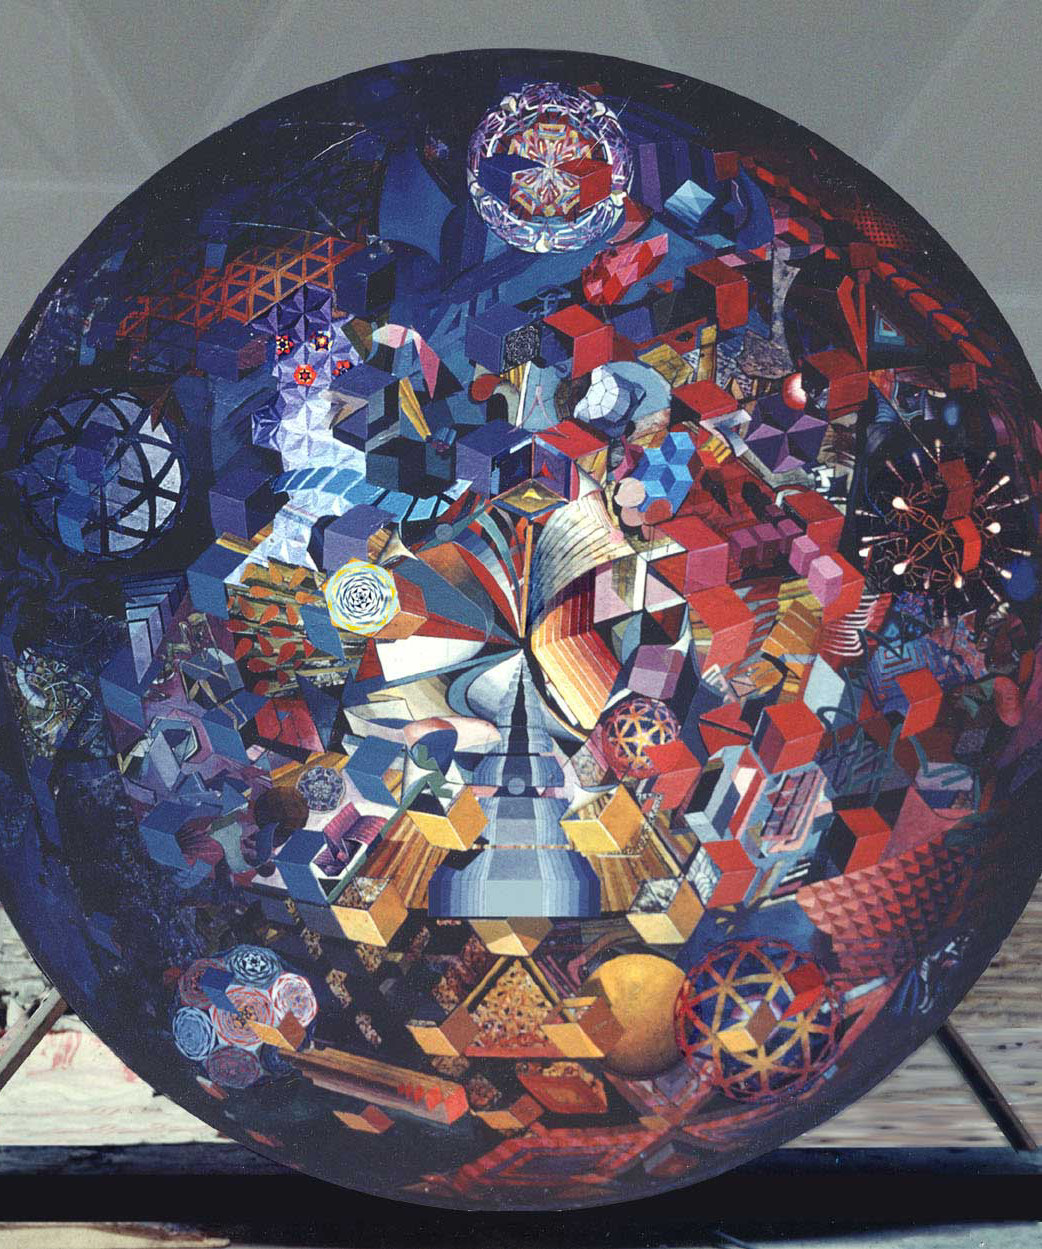
\includegraphics[width=\textwidth]{media/cubism_the_ultimate_painting_small.jpg}
	\end{columns}
\end{frame}

\videoframe[webm]{visual_cortex}{KE952yueVLA}

\videoframe[webm]{hippocampal_place_cells}{lfNVv0A8QvI}

\begin{frame}{NEF Principle 1: Representation}
	\begin{mdframed}
		\textbf{NEF Principle 1 -- Representation}\\
		\emph{Groups} (\enquote{populations}, or \enquote{ensembles}) of neurons \emph{represent} represent values via nonlinear encoding and linear decoding.
	\end{mdframed}
\end{frame}

\begin{frame}{Lossless Codes}
	\vspace{0.5cm}
	\begin{columns}
		\column{0.6\textwidth}
		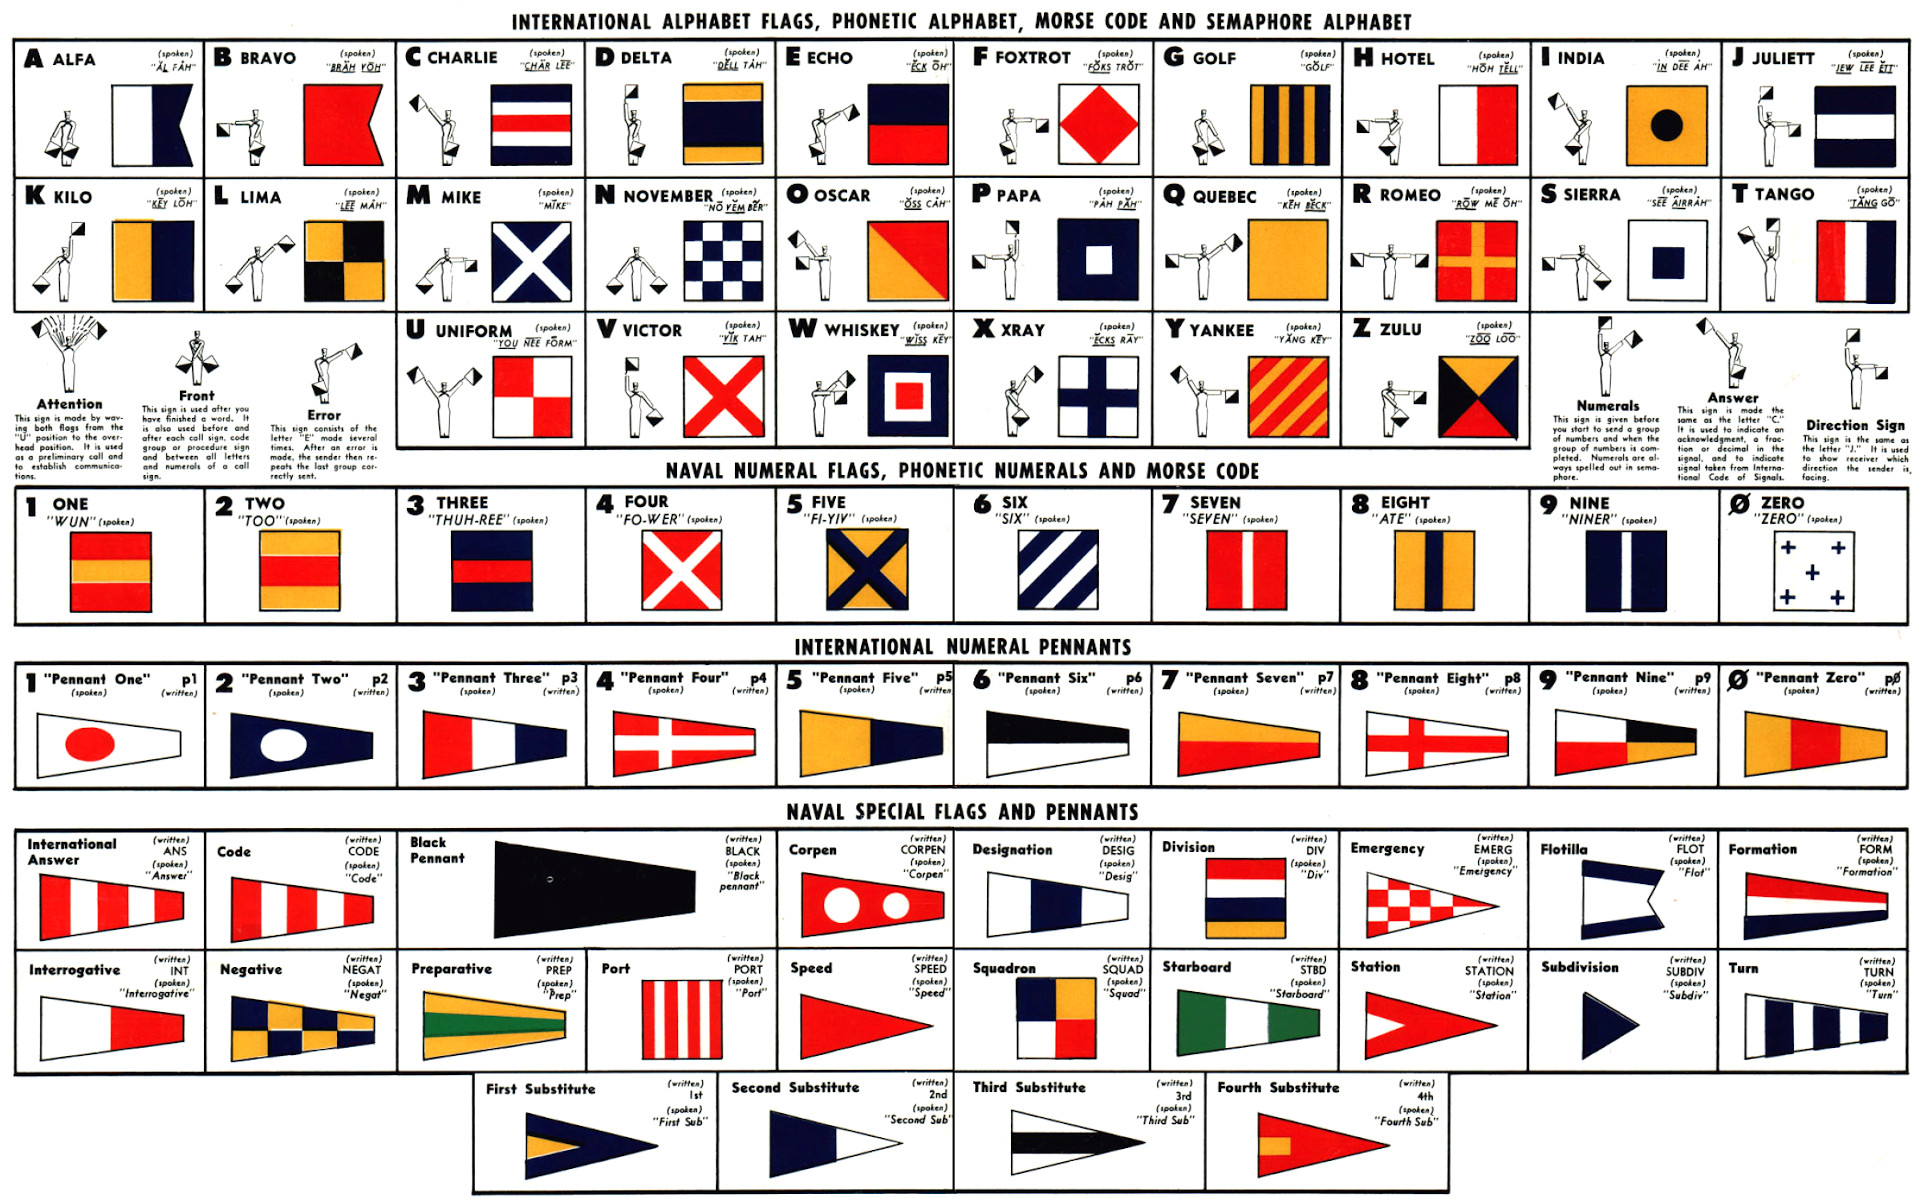
\includegraphics[width=\textwidth]{media/flag_alphabet_1956_small.jpg}
		\column{0.4\textwidth}
		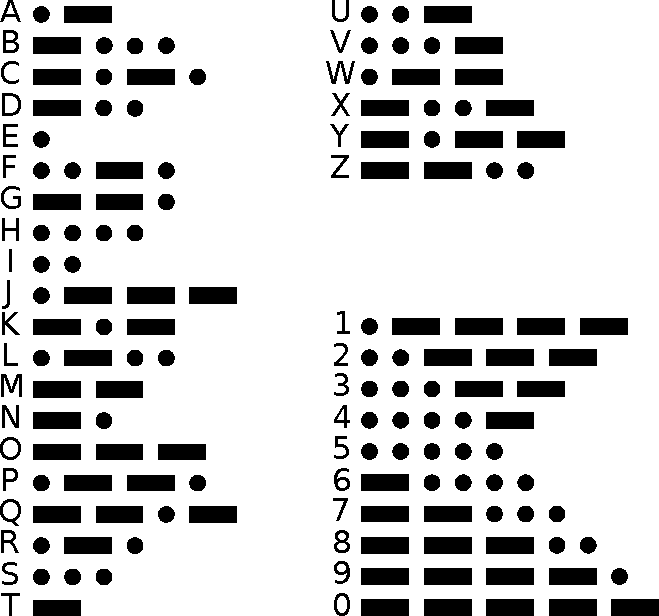
\includegraphics[width=\textwidth]{media/international_morse_code.pdf}
	\end{columns}
	\vspace{0.25cm}
	\begin{align*}
		\text{Encoding:} \quad \vec a &= f(\vec x) & \text{Decoding:} \quad \vec x &= f^{-1}(\vec a)
	\end{align*}
\end{frame}

\begin{frame}{Binary numbers: Nonlinear encoding, linear decoding}
	\begin{itemize}
		\setlength{\itemsep}{0.25cm}
		\item Represent a natural number between $0$ and $2^{n} - 1$ as $n$ binary digits.
		\item<2-> \textbf{Nonlinear encoding}
			\begin{align*}
			a_i &= \big(f(x)\big)_i = \begin{cases}
				1 & \text{if } x - 2^i \left\lfloor \frac{x}{2^i} \right\rfloor > 2^{i - 1} \,,\\
				0 & \text{otherwise} \,.
				\end{cases}
			\end{align*}
		\item<3-> \textbf{Linear decoding}\\[-1cm]
		\begin{align*}
			x &= f^{-1}(\vec a) = \sum_{i=0}^{n -1} 2^i a_i = \mat F \vec a = \begin{pmatrix} 1 & 2 & \ldots & 2^{n - 1}\end{pmatrix} \begin{pmatrix} a_0 \\ a_1 \\ \vdots \\ a_{n - 1} \end{pmatrix} \,.
		\end{align*}
		\item<4-> This is a \hl{distributed code}. \only<5->{But, \hl{not robust} against additive noise!}
	\end{itemize}
\end{frame}

\begin{frame}{Lossy codes}
	\begin{itemize}
		\setlength{\itemsep}{0.5cm}
		\item \textbf{Lossy code}\\
		Inverse $f^{-1}$ does not exist, instead \emph{approximate} the represented value
		\begin{align*}
			\text{Encoding:} \quad \vec a &= f(\vec x) & \text{Decoding:} \quad \vec x &\approx g(\vec a)
		\end{align*}
		\item<2-> \textbf{Examples}\\
		\begin{itemize}
			\setlength{\itemsep}{0.25cm}
			\item Audio, image, and video coding schemes\\(MP3, JPEG, H.264)\\
			\item Basis transformation onto first $n$ principal components (PCA)\\
			\item<3-> \textbf{Neural Representations}
		\end{itemize}
	\end{itemize}
\end{frame}

\begin{frame}{Tuning curves (I)}
	\begin{columns}
		\column{0.5\textwidth}
		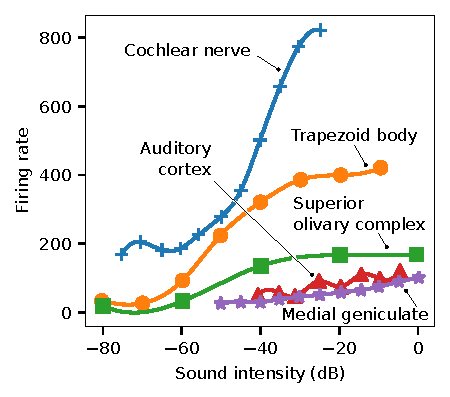
\includegraphics[width=\textwidth]{media/audition_tuning_curves_annotated.pdf}%
		\column{0.5\textwidth}
		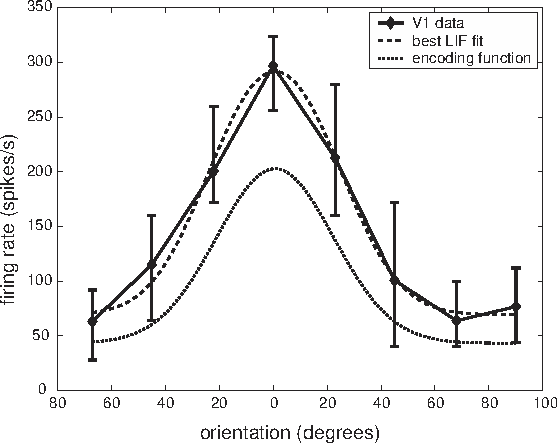
\includegraphics[width=\textwidth]{media/eliasmith_et_al_2003_orientation_tuning.pdf}%
	\end{columns}
\end{frame}

\begin{frame}{Tuning curves (II)}
	\begin{columns}
		\column{0.25\textwidth}
		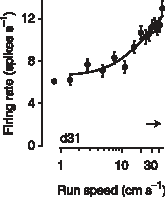
\includegraphics[scale=1.25]{media/saleem_et_al_tuning_curves_a.pdf}
		\column{0.25\textwidth}
		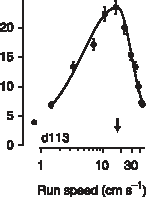
\includegraphics[scale=1.25]{media/saleem_et_al_tuning_curves_b.pdf}
		\column{0.25\textwidth}
		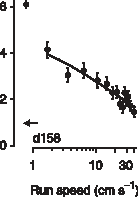
\includegraphics[scale=1.25]{media/saleem_et_al_tuning_curves_c.pdf}
		\column{0.25\textwidth}
		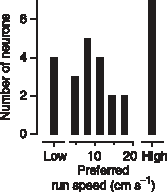
\includegraphics[scale=1.25]{media/saleem_et_al_tuning_curves_d.pdf}
	\end{columns}
\end{frame}

\begin{frame}{Preferred Directions in Higher Dimensions: Representing 2D Values}
	\begin{columns}[c]
		\column{0.5\textwidth}
		\centering
		\includegraphics<1->[height=5.75cm,trim=1cm 0cm 0cm 1cm,clip]{media/2d_encoder_tuning_curve.pdf}
		\column{0.5\textwidth}
		\centering
		\includegraphics<2->[height=5.75cm]{media/2d_encoder_tuning_curve_unit.pdf}	
	\end{columns}
\end{frame}

\begin{frame}{Decoding Without Taking Noise Into Account}
	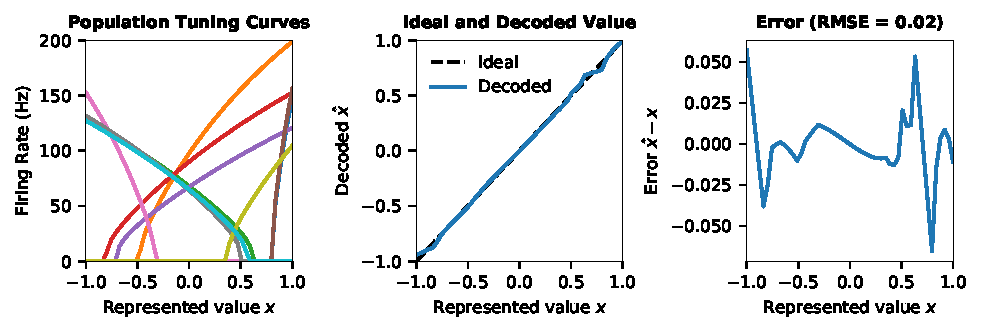
\includegraphics[width=\textwidth]{media/decoding_example_no_noise.pdf}
\end{frame}

\begin{frame}{Decoding Noisy $\mat A$ Without Taking Noise Into Account}
	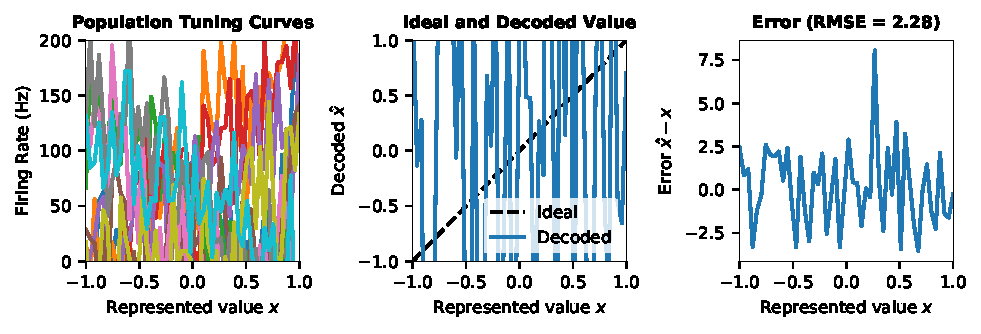
\includegraphics[width=\textwidth]{media/decoding_example_noise.pdf}
\end{frame}

\begin{frame}{Decoding Noisy $\mat A$ Accounting for Noise}
	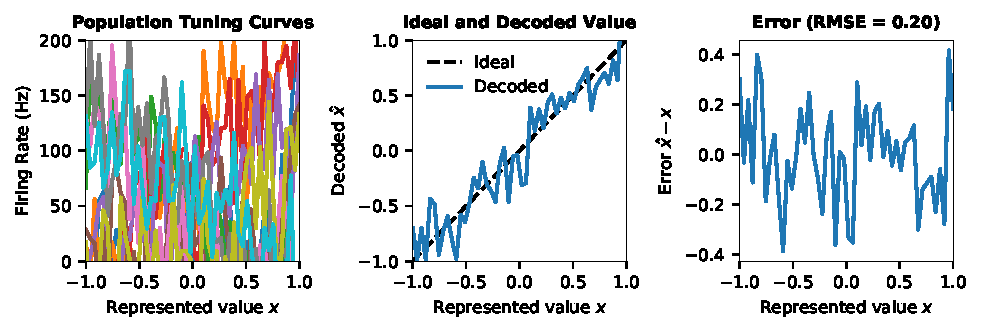
\includegraphics[width=\textwidth]{media/decoding_example_noise_accounted.pdf}
\end{frame}

\backupbegin

\begin{frame}{Administration}
	\begin{itemize}
		\setlength{\itemsep}{0.75cm}
		\item \hl{Assignment 1 has been released.}\\[0.25cm]
		The due date has been adjusted to January,~30.
		\item Some new potential times for office hours\\[0.5cm]
			\texttt{Mon 15:30-16:30}, \texttt{Mon 16:30-17:30}, \texttt{Tue 15:00-16:00},\\[0.5cm]
			\texttt{Thu 11:30-12:30} (current slot),\texttt{Thu 12:30-13:30}
	\end{itemize}
\end{frame}

\begin{frame}[noframenumbering]{Image sources}
	\small
	\textbf{Title slide}\\\enquote{The Ultimate painting.}\\Author: Clark Richert.\\From \href{https://commons.wikimedia.org/wiki/File:\%22The_Ultimate_painting\%22.jpg}{Wikimedia}.
\end{frame}


\backupend

\end{document}
